%%
%%
\documentclass[preprint,3p,10pt,number,sort&compress]{elsarticle}
%\documentclass[preprint,3p,10pt,twocolumn,number,sort&compress]{elsarticle}
%\documentclass[final,3p,10pt,twocolumn,number,sort&compress]{elsarticle}

%% if you use PostScript figures in your article
%% use the graphics package for simple commands
%% \usepackage{graphics}
%% or use the graphicx package for more complicated commands
 \usepackage{graphicx}
 \usepackage{amsmath}
 \usepackage{stfloats}
 \usepackage{afterpage}
 \usepackage{placeins}
 \usepackage{comment}
% \usepackage{xfrac}

%% or use the epsfig package if you prefer to use the old commands
%% \usepackage{epsfig}

%% The amssymb package provides various useful mathematical symbols
\usepackage{amssymb}
\usepackage{color}
%% The amsthm package provides extended theorem environments
%% \usepackage{amsthm}

%% The lineno packages adds line numbers. Start line numbering with
%% \begin{linenumbers}, end it with \end{linenumbers}. Or switch it on
%% for the whole article with \linenumbers after \end{frontmatter}.
%% \usepackage{lineno}

%\journal{Journal of Nuclear Materials}
\usepackage{lipsum}
\makeatletter
\def\ps@pprintTitle{%
 \let\@oddhead\@empty
 \let\@evenhead\@empty
 \def\@oddfoot{}%
 \let\@evenfoot\@oddfoot}
\makeatother
\begin{document}

\begin{frontmatter}

\title{KCl-UCl$_3$ molten salts investigated by \textit{Ab Initio} Molecular Dynamics (AIMD) simulations}

%\title{Mixing energies, heat capacities and densities of KCl-UCl$_3$ molten salts: \textit{Ab initio} molecular dynamics (AIMD) simulations}

\author[label1]{D. A. Andersson}
\ead{andersson@lanl.gov}
\author[label1]{G. Wang}
\author[label1]{P. Yang}
\author[label2,label3]{B. W. Beeler}

\address[label1]{Materials Science and Technology Division, Los Alamos National Laboratory P.O. Box 1663, Los Alamos, NM 87545, USA}
\address[label2]{Department of Nuclear Engineering, North Carolina State University, Raleigh, NC, United States}
\address[label3]{Idaho National Laboratory, Idaho Falls, ID 83415, United States}


\begin{abstract}

\textit{ab initio} Molecular Dynamics (AIMD) simulations are performed on molten KCl-UCl$_3$ salt mixtures to determine energies, heat capacities, and densities. 
The density-dependent energy correction (DFT-dDsC), Grimme et al.'s DFT-D3, and Langreth \& Lundqvist (vdW-cx) models are used for dispersion forces and combined with the Perdew-Burke-Ernzerhof (PBE) exchange-correlation potential with a Hubbard $U$ parameter for the 5$f$ electrons of uranium. After validating predictions for the end-member systems to literature data, KCl-UCl$_3$ mixtures are studied at select temperatures. Densities and energies both deviate from ideal solution behavior, with the maximum deviation occurring around 36\% UCl$_3$ for mixing energies and slightly lower (29\% UCl$_3$) for densities. Compared to the NaCl-UCl$_3$ system, which was previously investigated using the same simulation methodologies, the KCl-UCl$_3$ density and mixing energy deviations from ideal solution behavior are larger by almost a factor of two. %by about 50 \% .  
It is not possible to identify any deviation from ideal solution behavior for heat capacity. The AIMD predictions for mixing energies and densities agree qualitatively with experimental data, though the spread in data obtained from the various dispersion force models utilized, measurements, and empirical estimates makes strong conclusions difficult. The dependence of thermodynamic and thermophysical properties on composition is correlated with the local chemistry of the solution phase, in particular, the tendency of UCl$_3$ to form network structures.  
\end{abstract}

%\begin{keyword}
%% keywords here, in the form: keyword \sep keyword

%% MSC codes here, in the form: \MSC code \sep code
%% or \MSC[2008] code \sep code (2000 is the default)

%\end{keyword}

\end{frontmatter}

%%
%% Start line numbering here if you want
%%
% \linenumbers

%% main text
\section{Introduction}
\label{sec:intro}
Molten salts are proposed for use as fuel, heat transfer liquid, and a heat storage medium in Generation IV nuclear reactors and reactor systems~\cite{SERP2014308}. Traditional molten salt reactor (MSR) designs simultaneously use a molten salt as the heat transfer liquid and fuel by dissolving actinides into the salt. Alternatively, the fuel can be contained in TRISO particles dissolved in the molten salt, as in Fluoride-Salt-Cooled High-Temperature Reactors (FHRs)~\cite{jiang2022}. Oak Ridge National Laboratory (ORNL) built and operated the Molten Salt Reactor Experiment (MSRE)~\cite{MSRE1,MSRE2} in the 1960s, which used a fluoride salt (FLiBe) with uranium as fuel. Today, both fluoride and chloride salts are being considered for advanced MSR designs by companies and research organizations. The strong interest in MSRs has revitalized the need for accurate properties of pure and mixed salts. The present study targets fuel-containing salts by calculating mixing energies, heat capacities, and densities of one of the chloride systems, KCl-UCl$_3$, considered for MSRs in the fast neutron spectrum, either on its own or mixed with other base salts, such as NaCl or MgCl$_2$. \textit{Ab Initio} Molecular Dynamics (AIMD) simulations are used for this purpose. The goal is to provide new data points that can be used in combination with experiments to develop databases of thermochemical~\cite{ARD2022153631} and thermophysical~\cite{BIRRI2022117954} properties. The atomic scale simulations also allow the linkage of macroscale properties to the local atomic structure of salts, thus improving the fundamental understanding.   

The temperature-dependent density and heat capacity of KCl are available from experimental literature studies, as collected by Janz \cite{Janz1988} and originally reported by van Artsdalen and Yaffe,~\cite{Artsdalen1955}.  As part of studies of the LiCl-KCl system, Duemmler \textit{et al.}~\cite{DUEMMLER2022153414} and Bengtson \textit{et al.}~\cite{BENGTSON2014362} investigated the temperature-dependent properties of KCl by AIMD simulations. Their results are in good agreement with both historic experimental data and new measurements~\cite{Artsdalen1955,DUEMMLER2022153414}. The heat capacity of KCl is available in databases~\cite{NIST,219851}. The density of the UCl$_3$ end-member salt was studied by Parker \textit{et al.}~\cite{Parker} using neutron imaging experiments. Their results were noticeably different from older experiments performed by Desyatnik \textit{et al}!~\cite{Desyatnik2}. The results of Parker \textit{et al.}~\cite{Parker} were confirmed by AIMD simulations~\cite{Andersson}. The heat capacity of UCl$_3$ is not available directly from experiments, but it has been estimated in a CALPHAD assessment~\cite{YIN2020,BENES2008} and it has also been calculated by AIMD simulations~\cite{Andersson}.
 
The density, heat capacity, and viscosity of KCl-UCl$_3$ mixtures were recently reported by Moon \textit{et al.}~\cite{Moon} from neutron imaging experiments. Experimental densities were earlier reported by Desyatnik \textit{et al.}~\cite{DesyatnikKCl}, which deviates by up to $\approx 5$\% from the more recent study. Can \textit{et al.} collected experimental data and developed models of the KCl-UCl$_3$ thermophysical properties based on a Redlich-Kister expansion~\cite{agca2022}. Kim \text{et al.}~\cite{Kim} used molecular dynamics (MD) simulations to calculate the density, heat capacity, and viscosity of KCl-UCl$_3$ mixtures. The mixing energy of KCl-UCl$_3$ was reported by Rycerz \textit{et al.}~\cite{Rycerz}. There are also several thermodynamic assessments and empirical estimates of the mixing energy, which in some cases agree well with the experimental data~\cite{Rycerz,Yingling} and in some cases exhibit variations~\cite{YIN2020,Ghosh}. The empirical value used in the CALPHAD assessments by Yin et al.~\cite{YIN2020} and Ghosh \textit{et al.}~\cite{Ghosh} are within $\approx 31$\% (smaller) and $\approx 35$\% (larger) of the experimental measurements by Rycerz \textit{et al.}~\cite{Rycerz}, respectively. Yingling \textit{et al.}~\cite{Yingling} had access to the experimental data on mixing energies in their CALPHAD assessment, but also compared them to an empirical estimate by Schorne-Pinto \textit{et al.}~\cite{Pinto}. The latter estimate is within $\approx 14$\% of the experimental value. Compared to the closely related NaCl-UCl$_3$ system, existing data indicate that KCl-UCl$_3$ densities and mixing energies deviate more significantly from an ideal solution behavior, which is expected based on the larger size of K ions compared to Na ions. This relationship is the basis of the correlations used for the empirical mixing energy estimates in the references above. 

The range of values reported for mixing energies and densities motivate the present AIMD simulations of KCl-UCl$_3$. AIMD simulations are used to predict a subset of thermophysical (density) and thermodynamic (mixing energy and heat capacity) properties. The AIMD simulations performed follow a similar approach as was previously applied to the analogous NaCl-UCl$_3$ system~\cite{Andersson} and also the LiCl-KCl system~\cite{DUEMMLER2022153414}. The remainder of this paper is organized as follows. The methodology is described in Sec. \ref{sec:method}, followed by results and discussion in Sec. \ref{sec:results}, which includes comparison to experiments and other molten salt systems, in particular NaCl-UCl$_3$. Finally, our conclusions are presented in Sec. \ref{sec:conclusions}. 

\section{Methodology}
\label{sec:method}
\subsection{Density functional theory}
The AIMD simulations are based on density functional theory (DFT) and utilize the VASP code~\cite{Kresse1996}.
Isobaric (NPT) conditions are imposed for all simulations (with the pressure set to zero) to evaluate density, thermal expansion, heat capacity, and mixing energy. All simulations used the Langevin thermostat in VASP with the temperature friction coefficient set to 10 ps$^{-1}$ and the friction coefficient for the lattice degrees of freedom to 1 ps$^{-1}$. The time step is 2 fs for production runs between 1100 K and 1500 K. For temperatures lower than 1100 K, a 5 fs time step is used. For each temperature and composition, simulations are performed for at least 20 ps in order to equilibrate the system. After equilibration, production simulations are performed for a minimum of 30 ps, often longer. NPT simulations sometimes require long equilibration times and may leave the equilibrium state due to (significant) distortions of the supercell. This is likely a consequence of the somewhat small supercells. These regimes typically correspond to a noticeably higher energy. For reliable results, sampling of such regimes is avoided.

Properties are calculated by averaging the AIMD results over the production simulation time. Densities are obtained from the supercell volume and the heat capacities at constant pressure are obtained from the slope of the total internal energy ($E_{tot}$) as a function of temperature:
\begin{equation}
\label{eq:cp}
C_p=\frac{\partial E_{tot}}{\partial T}
\end{equation}
The pressure is enforced to be zero in our calculations. 
Mixing energies of U$_x$K$_y$Cl$_{3x+y}$ were referenced to pure KCl and UCl$_3$ at the same temperature and calculated from the potential energy ($E_{pot}$):
\begin{equation}
\begin{split}
E_{mix}=E_{pot}(U_xK_yCl_{3x+y})-xE_{pot}(UCl_3)-yE_{pot}(KCl).
\end{split}
\end{equation}
The mixing energy is defined per formula unit, or equivalently per cation. 

For simulations with the DFT-dDsC dispersion correction, the KCl and UCl$_3$ simulations use supercells of 64 atoms, and the mixed KCl-UCl$_3$ systems contain between 60 and 76 atoms and are inherited from the NaCl-UCl$_3$ system~\cite{Andersson}. Convergence tests and other simulation cell characteristics are provided in Ref.~\cite{Andersson}. For simulations with the vdW-cx non-local functional, supercells contain between 88 and 112 atoms and were created by the Packmol package~\cite{packmol}. Even though there is variation in the supercell sizes used in the simulations, the results are sufficiently converged for all cases to support the data and conclusions of the present study. For computational efficiency, integration in reciprocal space only uses the $\Gamma$ point. The accurate simulation setting is utilized in VASP, but the plane wave cut-off energy is increased above the standard setting to 400 eV. The partial occupancies of the wave functions are described by Gaussian smearing with a smearing parameter of 0.05 eV. The convergence criteria for the electronic minimization is 10$^{-3}$ eV for KCl and $5\times10^{-3}$ eV for salts containing uranium. The properties of interest are converged for both settings~\cite{Andersson}. The Projector Augmented Wave (PAW) method is used to describe the core electrons~\cite{PAW1,PAW2}. The PAW potentials supplied with VASP for the PBE exchange-correlation potential are utilized. For K, the potential version that includes both the $s$ and the semi-core $p$ electrons ($2p^63s^1$) is chosen. The PAW potential for Cl also includes $p$ electrons ($3s^2p^5$) and for U it includes the outer $s$, $p$, $d$, and $f$ electrons ($6s^26p^65f^36d^17s^2$) in the valance shell. The generalized gradient approximation (GGA) with a Hubbard $U$ parameter is used to describe the strongly correlated $f$ electrons of uranium~\cite{Andersson}. Ref. ~\cite{Andersson} determined that a $U$ value of 4.5 eV and a $J$ value of 0.51 eV (or a $U_{eff}$ value of 4 eV) are appropriate for the UCl$_3$ system. The magnetic moments on uranium ions are aligned in an approximate AFM pattern, mimicking a random distribution of spins consistent with the prevailing distribution in high-temperature molten salts. Non-spherical contributions related to the gradient of the density in the PAW spheres are included and LMAXMIX is increased to 6 to include $f$-electrons in the charge density mixing routines. 

Dispersion interactions are included in the DFT simulations using a couple of methods. Following the study in Ref.~\cite{Andersson}, the density-dependent energy correction (DFT-dDsC)~\cite{Steinmann2011,Steinmann2} method is applied. An updated version of the Langreth \& Lundqvist method (vdW-cx)~\cite{Dion2004,Klimes2010,Perez2009,Berland2014} is applied, whereas the vdW-DF2 formalism was utilized for the NaCl-UCl$_3$ system. This change was motivated by the discrepancies in thermal expansion of UCl$_3$ rich systems as predicted by the vdW-DF2 functional, and the positive performance of the vdW-cx functional for water \cite{Torres2021}, a variety of covalent molecules \cite{Berland2017}, and even numerous solids \cite{Tran2019}. Additionally, the DFT-D3 method by Grimme et al.~\cite{Grimme} is utilized for KCl for select mixed salt cases. The DFT-dDsC method does not include parameters for $f$ elements in the standard VASP version. The parameters are taken from Kim~\cite{Kim} ($C_6$=4.889 au and $r_0$=6.416 au) and Schwerdtfeger~\cite{pol} ($\alpha$=129.0 au).

\section{Results and discussion}
\label{sec:results}

\subsection{Density and heat capacity of KCl and UCl$_3$ end-member molten salts}
\label{sec:endmember}
The thermo-physical properties of KCl have been investigated by simulations and experiments~\cite{Janz1988,Artsdalen1955,Moon,DUEMMLER2022153414}. Data and correlations for density are collected in Figure \ref{fig:KCl}, which also includes the present AIMD results using the DFT-dDsC, vdW-cx, and DFT-D3 dispersion force models. The experimental data is consistent between references and exhibits small scatter. The DFT-D3 and DFT-cx dispersion force models both agree with the experimental data within $\approx 2$ \% in the temperature range where the experimental data was collected, though the temperature dependence in the simulations is slightly different than in the experiments. The DFT-dDsC model predicts densities that are $\approx 4$\% lower than the experimental data, with a temperature dependence that is somewhat closer to experiments than the other dispersion force models. The comparison between computational and experimental results for KCl is shifted down from the NaCl case~\cite{Andersson}, for which the predicted densities were consistently higher than experimental measurements. The dashed lines in Figure \ref{fig:KCl} are linear least-squares fits to the calculated data points. The resulting correlations for density are listed in Table \ref{table:KCldensityetc} together with the corresponding information from literature experiments and simulations. 

\begin{figure}[h!]
\centering
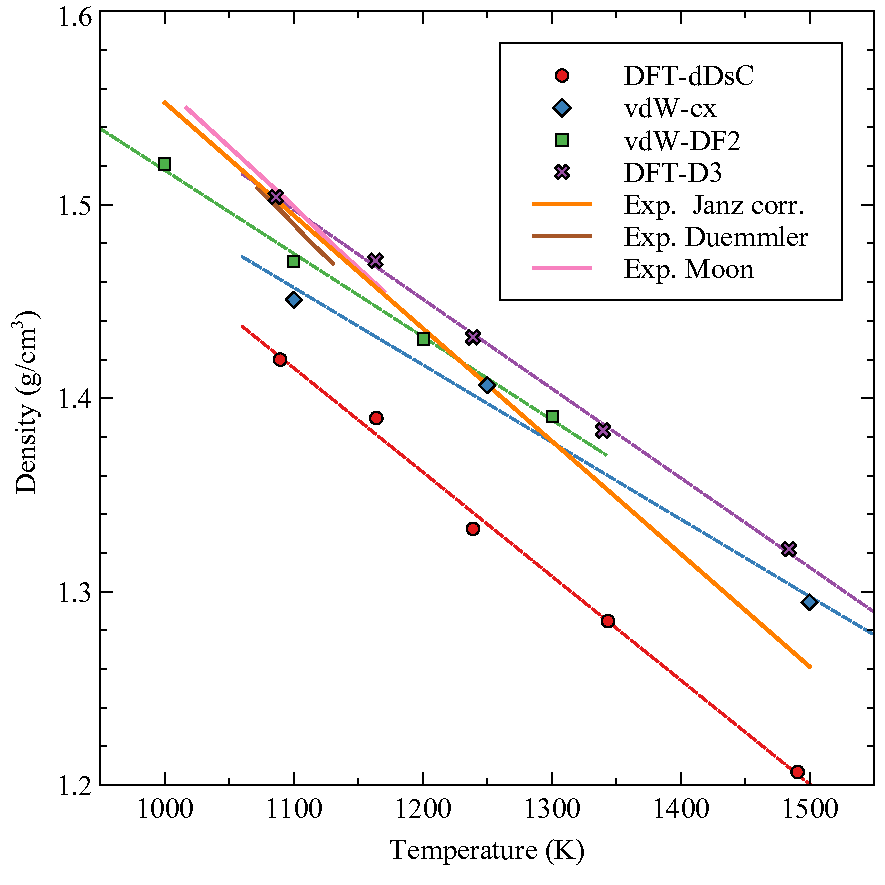
\includegraphics[width=0.45\textwidth]{ben_fig1.pdf}
\caption{Calculated density of KCl as a function of temperature obtained using different methods to describe dispersion force interactions (DFT-dDsC, vdW-cx, DFT-D3), compared to experimental data (Moon \textit{et al.}~\cite{Moon} and Duemmler \textit{et al.}~\cite{DUEMMLER2022153414}) or correlations (Janz~\cite{Janz1988}). The computational data from 
from Duemmler \textit{et al.}~\cite{DUEMMLER2022153414} for the vdW-DF2 is also shown. The dashed lines are least-squares fits to calculated data points.} 
\label{fig:KCl}
\end{figure}

\begin{table*}[hb!]
\centering
\caption{Calculated and experimental correlations and values for density and heat capacity (C$_p$) of KCl. Where known, the temperatures within parenthesis indicate the range of data used for fitting the models from either AIMD simulations or experiments.}
\begin{tabular}{lcc}
\hline
\hline
& Density (g/cm$^3$) &Heat capacity (J/mol/K) \\
\hline
KCl Calculated (DFT-dDsC)	&$2.0149-0.0005432T$ ($1100 - 1500$ K) &75.4 ($1100 - 1500$ K)\\
KCl Calculated (vdW-cx)	& $1.8933-0.0003968T$ ($1100 - 1500$ K)& 71.1 ($1100 - 1500$ K)\\
KCl Calculated (DFT-D3)	&2.0070-0.0004630T ($1100 - 1500$ K)& 70.4 ($1100 - 1500$ K)\\
KCl Experiment	&$2.1359-0.0005831 T$~\cite{Janz1988} ($1053-1212$ K) &73.6~\cite{NIST} \\	
\hline
\hline
\end{tabular}
\label{table:KCldensityetc}
\end{table*}

The simulations predict a constant heat capacity in the temperature range investigated. Literature and calculated heat capacities of KCl are presented in Table \ref{table:KCldensityetc}. There is very good agreement between all calculations and experimental data. 

The properties of UCl$_3$ obtained from DFT-dDsC simulations were previously reported~\cite{Andersson} and the results will not be repeated here. The vdW-cx formalism nearly exactly reproduces the densities at 1100 K and 1250 K, while predicting a higher value for the density at 1500 K. With this limited dataset, the thermal expansion predicted by the vdW-cx underestimates the values predicted from experiment and from the DFT-dDsC correction. The main conclusion in the context of the present study is that the level of agreement for the various dispersion force models with experimental densities of UCl$_3$ is not the same as for KCl. Rather the most accurate prediction for density was obtained by the DFT-dDsC model. This highlights the challenges of obtaining quantitative predictions of thermo-physical properties for actinide-containing mixed molten salts. For this reason, we choose to include multiple dispersion force models in the investigation of the mixed KCl-UCl$_3$ system. Heat capacities of UCl$_3$ from both the DFT-dDsC (141.4 J/mol-K~\cite{Andersson}) and vdW-cx (136.9 J/mol-K) models of dispersion force interactions are predicted to be within the range of reported experimental values (129.8 J/mol-K~\cite{YIN2020}, 150 J/mol-K~\cite{BENES2008}).

\subsection{Energies and heat capacities of mixed KCl-UCl$_3$ salts}
For the DFT-dDsC/vdW-cx methods, the KCl-UCl$_3$ mixing energies are calculated at 7/8 compositions and three different temperatures, 1100 K, 1250 K, and 1500 K, with the pure KCl and UCl$_3$ end-members as references. The DFT-D3 method is only used at a single temperature, 1250 K. The results are shown in Figure \ref{fig:KCl_UCl3_energy}a) at 1250 K, which also includes experimental reference values~\cite{Rycerz}, CALPHAD assessments~\cite{YIN2020,Ghosh}, and data from (semi-)empirical correlations~\cite{Pinto}. 
Figure \ref{fig:KCl_UCl3_energy}b) shows a comparison to previously calculated values for the analogous NaCl-UCl$_3$ system~\cite{Andersson} at different temperatures. {\color{red} (i removed the different temperature data from fig2a because it just became too many datasets. i think showing the temperature dependence in fig2b suffices here)} 
Similar to the NaCl-UCl$_3$ system, the mixing energy is a minimum at $\approx~36$\% UCl$_3$, which is close to the eutectic composition in the NaCl-UCl$_3$ phase diagram ($\approx 35$\% UCl$_3$). Strictly, the simulations pinpoint the minimum to occur between $36$\% and $50$\% UCl$_3$, but the composition trend favors the lower end of this range as the minimum. Note that the same eutectic composition in the KCl-UCl$_3$ system is hidden due to the presence of the K$_2$UCl$_5$ line compound (corresponding to $\approx~33$\% UCl$_3$), nevertheless, it is reasonable to expect that a eutectic would be present at this composition in a meta-stable phase diagram that suppresses the formation of the solid K$_2$UCl$_5$ phase. As shown in Figure \ref{fig:KCl_UCl3_energy}b, the DFT-dDsC simulations indicate that, within the uncertainties of the simulations, the mixing energy is independent of temperature, as in the NaCl-UCl$_3$ system. The vdW-cx simulations, although not shown, agree with this observation.  

\begin{figure*}[h!]
\centering
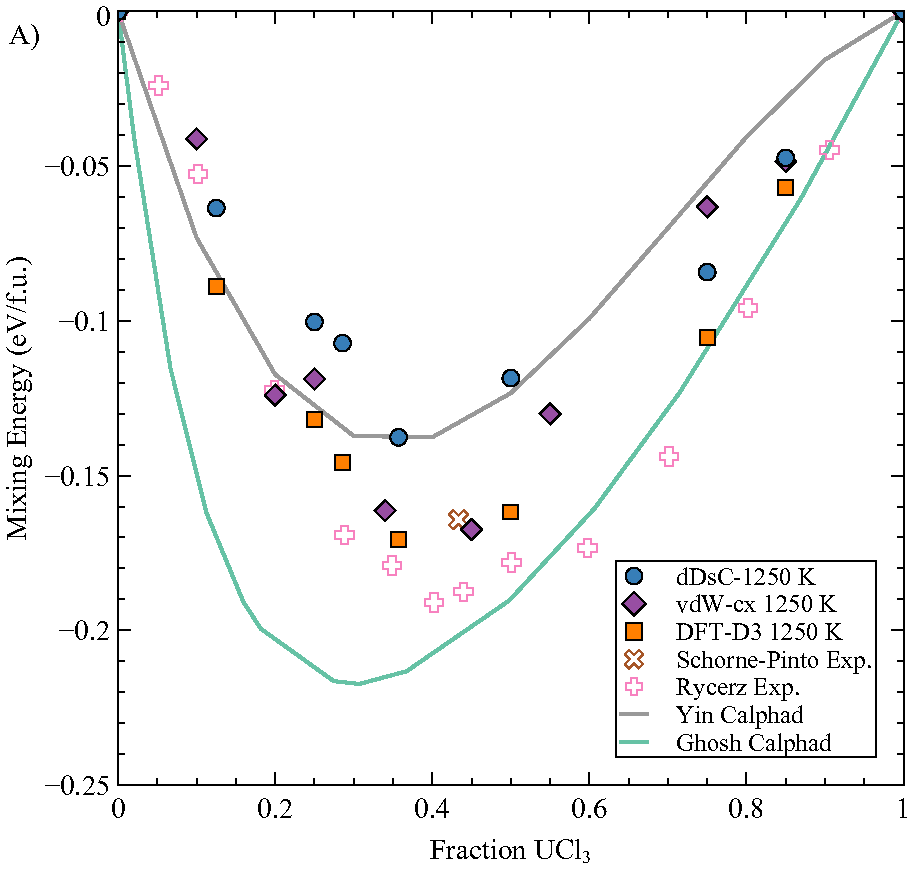
\includegraphics[width=0.45\textwidth]{ben_fig2a.pdf}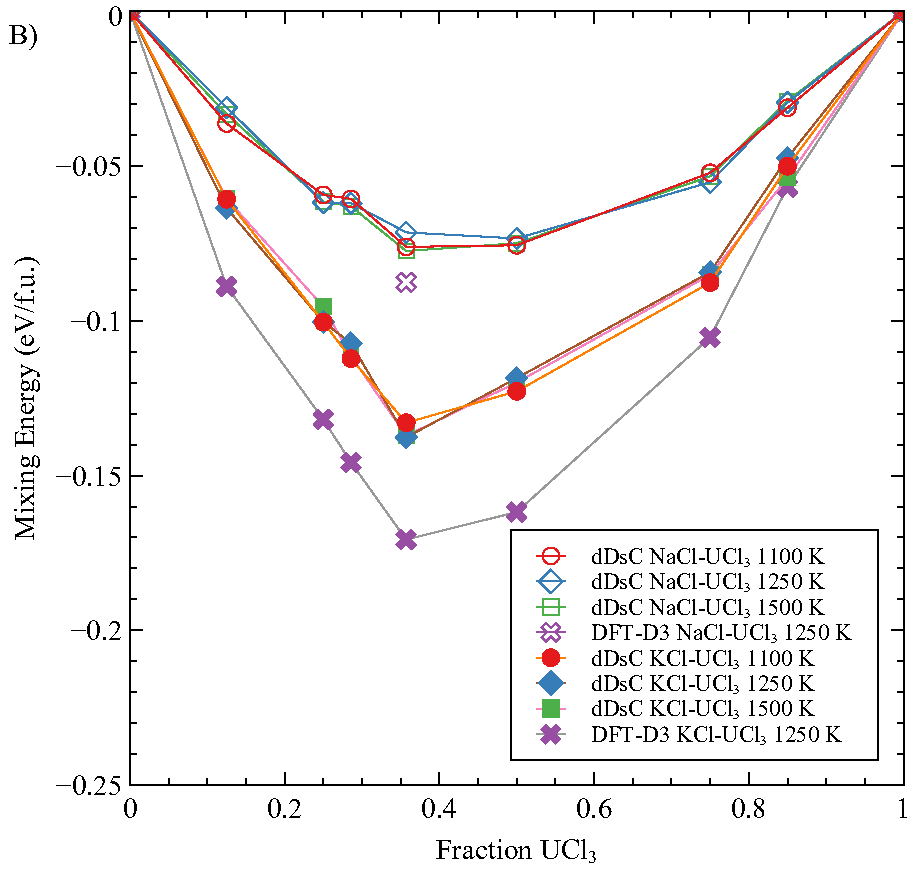
\includegraphics[width=0.45\textwidth]{ben_fig2b.pdf}
\caption{a) Mixing energies of KCl-UCl$_3$ calculated by the DFT-dDsC and DFT-DF2 methods at 1100 K, 1250 K and 1500 K and DFT-D3 at 1250 K. Experimental reference values~\cite{Rycerz}, predictions from CALPHAD models~\cite{YIN2020,Ghosh}, data from (semi-)empirical correlations~\cite{Pinto}. b) Calculated KCl-UCl$_3$ mixing energies compared to previously calculated DFT-dDsC values for the analogous NaCl-UCl$_3$ system~\cite{Andersson} and a new data point using the DFT-D3 method. }
\label{fig:KCl_UCl3_energy}
\end{figure*}

The shape of the mixing energy curve as a function of composition is similar to the NaCl-UCl$_3$ case, but the magnitude of the mixing energy is larger by almost a factor of two. The more negative mixing energy of KCl-UCl$_3$ as compared to NaCl-UCl$_3$ is expected based on empirical correlations relating the mixing energy to the ionic size of K$^{1+}$ (larger) and Na$^{1+}$ (smaller) to that of U$^{3+}$~\cite{YIN2020,Pinto}. The vdW-cx simulations confirm the DFT-dDsC shape of the mixing energy curve as a function of composition, but the energies are lower by a little over 20\%. The DFT-D3 simulations agree quite closely with the vdW-cx results. Although only a single temperature was investigated for the DFT-D3, the lack of discernible temperature dependence for the other simulation methods means that the T=1250 K case can be viewed as representative of a larger temperature range. In order to better understand the lower DFT-D3 mixing energy, a point calculation was performed for the NaCl-UCl$_3$ system at 36\% UCl$_3$ with the DFT-D3 method. This allows a comparison with the values reported in the literature for this system based on the DFT-dDsC method~\cite{Andersson}. 
The DFT-D3 mixing energy of NaCl-UCl$_3$ at 1250 K was calculated to be -0.088 eV/f.u., which is about 20\% lower than the DFT-dDsC prediction (-0.074 eV/f.u.)~\cite{Andersson}. Correspondingly, the vdW-DF2 dispersion formalism (utilized as a proxy for the vdW-cx formalism in this case) predicted the minimum mixing energy for the NaCl-UCl$_3$ system to be approximately -0.087 eV/f.u. This suggests that the lower mixing energies obtained for KCl-UCl$_3$ with the vdW-cx and DFT-D3 as compared to the DFT-dDsC method derive from the difference between the dispersion force models, and appear to be consistent across different UCl$_3$ mixed systems. 

The following expression is fitted to the KCl-UCl$_3$ mixing energy as a function of composition and temperature:
\begin{equation}
\begin{split}
E_{mix}(x,T)=(e_1+e_2T)x(1-x)+(f_1+f_2T)x(1-x)(2x-1),
\label{eq:LSE}
\end{split}
\end{equation}
where the parameters for all the temperature-dependent terms are set to zero based on the lack of discernible temperature dependence in Figure \ref{fig:KCl_UCl3_energy}. This expression is equivalent to the Redlich-Kister expansion used in existing CALPHAD models. The coefficients resulting from the fit to the DFT-dDsC data in Figure \ref{fig:KCl_UCl3_energy} are summarized in Table \ref{table:LS}. 

\begin{table}[hb!]
\centering
\small
\caption{A least-squares fit of the coefficients describing density and mixing energy of the KCl-UCl$_3$ system with the DFT-dDsC dispersion model as a function of temperature, see Eqs. \ref{eq:LSE} and \ref{eq:LS}.{\color{red} should my vdW-cx data be included here? or the DFT-D3 data? would make for a big table...}}
\begin{tabular}{lcc}
\hline
\hline
&Density (Eq. \ref{eq:LS}) &Mixing energy (Eq. \ref{eq:LSE}) \\
\hline
$e_1$ &-1.8779 (g/cm$^3$) &-0.50144 (eV) \\
$e_2$ &0.0012398 (g/cm$^3$/K) &0 (eV/K)\\
$f_1$ &-0.88798 (g/cm$^3$) &0.11401 (eV) \\
$f_2$ &0.00092495 (g/cm$^3$/K) &0 (eV/K)\\
\hline
\hline
\end{tabular}
\label{table:LS}
\end{table}

The vdW-cx and DFT-D3 values are close to the experimental data due to Rycerz \textit{et al.}~\cite{Rycerz}, while the DFT-dDsC predictions are higher. For NaCl-UCl$_3$ the DFT-dDsC values were in excellent agreement with experimental data~\cite{Andersson}. The reason for this difference in behavior between simulations for NaCl-UCl$_3$ and KCl-UCl$_3$ is not clear nor is it not possible to state which of the AIMD approaches is more reliable. The result emphasizes that the AIMD predictions must be treated with uncertainties when they are used in thermodynamic assessments, just as experimental data points. 
The Rycerz \textit{et al.} data set was used as input to the CALPHAD assessment by Yingling \textit{et al.}~\cite{Yingling}, and the resulting thermodynamic model is stated to be in good agreement with the experimental data points. Several schemes have been developed to estimate the magnitude of the mixing energy based on the mismatch in ionic radii between the salt constituents. One example is the work of Schorne-Pinto \textit{et al.}~\cite{Pinto}, which also closely matches the vdW-cx and DFT-D3 predictions. {\color{red} I changed your analysis here. see if you agree}
Yin \textit{et al.}~\cite{YIN2020} used a related scheme in their CALPHAD assessment of the KCl-UCl$_3$ system, with the resulting mixing energy in very close agreement with the DFT-dDsC predictions and higher than the experimental data due to Rycerz \textit{et al.}~\cite{Rycerz}. Finally, the CALPHAD assessment of Ghosh \textit{et al.}~\cite{Ghosh} utilized an estimation that resulted in a noticeably different mixing energy curve. This assessment is significantly lower than any of the simulations and appears to be outside the expected range of uncertainty, both in the magnitude of the mixing energy curve and the location of the minimum with respect to composition. 

Within the uncertainties of the AIMD simulations, the total energy is a linear function of temperature for all simulation methods, which implies that heat capacity can be approximated by a constant value. The heat capacity as a function of composition is plotted in Figure \ref{fig:heat_capacity}. It follows a near linear relation across the composition range, which implies the mixture approximately behaves like an ideal solution from the point of view of heat capacity. This is consistent with the lack of temperature dependence for the mixing energies in Figure \ref{fig:KCl_UCl3_energy}. Small deviations from the linear relation occur in Figure \ref{fig:heat_capacity}, but given the uncertainties of the simulations across the composition range, we refrain from trying to assign the non-linear part to excess heat capacity. The simulation results due to Kim \textit{et al.}~\cite{Kim} based on a polarizable ion model are reproduced in Figure \ref{fig:heat_capacity}, which exhibits excellent agreement with the data generated by AIMD. A small deviation from ideal solution behavior would be expected based on the study of Redkin \textit{et al.}~\cite{Redkin}, which identified a correlation between negative mixing energies and excess heat capacity at the eutectic composition. The predicted heat capacity at 36\% UCl$_3$ is in qualitative agreement with the observation of Redkin \textit{et al.}~\cite{Redkin}. However, as mentioned above, one should be careful assigning this simulation result to anything other than statistical variation. The excess heat capacity may be derived as the derivative of Eq. \ref{eq:LSE}, but would be equal to zero due to the lack of clear temperature dependence in the simulations, as discussed above. The heat capacity of mixtures is given by a linear interpolation of the end members. 

\begin{figure}[h!]
\centering
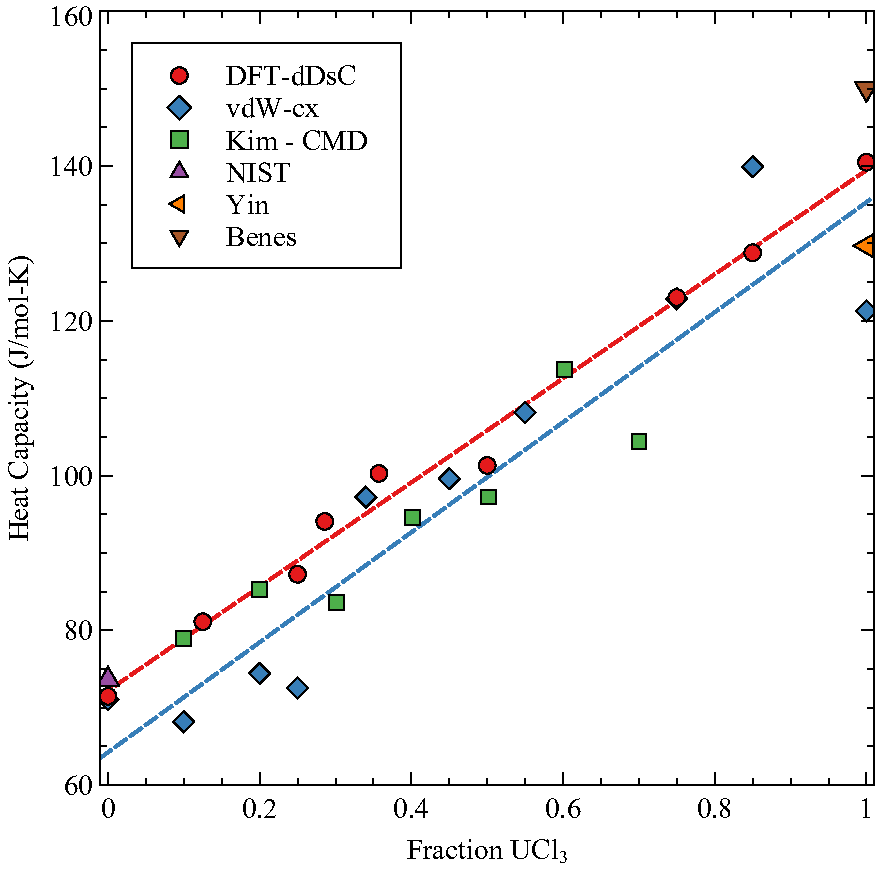
\includegraphics[width=0.45\textwidth]{ben_fig3.pdf}
\caption{Heat capacity as function of UCl$_3$ composition. The dashed line for the heat capacity represents a least-squares fit of a linear correlation. Literature experimental~\cite{NIST,219851,YIN2020,BENES2008} and computational data~\cite{Kim} are also shown.}
\label{fig:heat_capacity}
\end{figure}

\subsection{Densities of mixed KCl-UCl$_3$ molten salts}
The densities of mixed KCl-UCl$_3$ salts are plotted as a function of temperature in Figure \ref{fig:density}a for the DFT-dDsC, vdW-cx, and DFT-D3 models. Figure \ref{fig:density}b plots the deviation from ideal solution behavior derived from this data (the vdW-cx data is excluded in \ref{fig:density}b for legibility). This is a convenient way of visualizing the behavior of the mixed system since the absolute densities in Figure \ref{fig:density}a obscure the small but still important changes introduced by the interactions in the mixture. The density relations identified by the AIMD simulations can be expressed in a combined composition-temperature dependent correlation:
\begin{equation}
\begin{split}
\rho(x,T)=\frac{M_{KCl}(1-x)+M_{UCl_3}x}{\frac{M_{KCl}(1-x)}{\rho_{KCl}}+\frac{M_{UCl_3}x}{\rho_{UCl_3}}}+(e_1+e_2T)x(1-x)+(f_1+f_2T)x(1-x)(2x-1), 
\label{eq:LS}
\end{split}
\end{equation}
\noindent where the first term represents the density of an ideal solution and the subsequent terms the deviation from ideal solution behavior using a Redlich-Kister expansion. $M_{NaCl}$ and $M_{UCl_3}$ are the molar masses of the end-member salts, $\rho_{KCl}$ and $\rho_{UCl_3}$ are the temperature-dependent densities of the end-member salts taken from the correlations derived in Sec. \ref{sec:endmember} (KCl) and Ref.~\cite{Andersson} (UCl$_3$), $T$ is temperature, and $x$ is the mole fraction of UCl$_3$ in the mixture. This model follows the Redlich-Kister model used by Agca \textit{et al.} \cite{agca2022}. Table \ref{table:LS} summarizes the coefficients describing deviation from an ideal solution obtained from a least-squares fit of Eq. \ref{eq:LS} to the calculated DFT-dDsC data points. The densities from the vdW-cx closely match those of the DFT-dDsC formalism across the entire temperature and compositional range, and thus an additional fitting to the vdW-cx data was not included. The fit captures the absolute densities well, but cannot reproduce all the features of the deviation from ideal solution behavior (not shown), which is due to the sharp transition at x=0.29 and the stronger temperature dependence exhibited in the UCl$_3$-rich range.

The deviation from ideal solution behavior was measured by Desyatnik \textit{et al.}~\cite{DesyatnikKCl} across several compositions and temperatures, from which correlations were derived that were used to calculate the experimental data points shown in Figure \ref{fig:density}a. The measurements are in qualitative agreement with the AIMD predictions, with calculations showing a maximum deviation from ideal solution behavior close to 29\% UCl$_3$. The magnitude of the maximum deviation is 3 to 5 \% with decreasing values for increasing temperatures, which is similar to the experimental results. The experiments also capture the positive deviation occurring close to UCl$_3$ at 1500 K. Following the more negative mixing energies for KCl-UCl$_3$ as compared to NaCl-UCl$_3$, the deviation from ideal solution behavior exhibits values that are more negative for KCl-UCl$_3$ than for NaCl-UCl$_3$ by approximately a factor of two. However, the trends are very similar between the two systems. 

\begin{figure*}[h!]
\centering
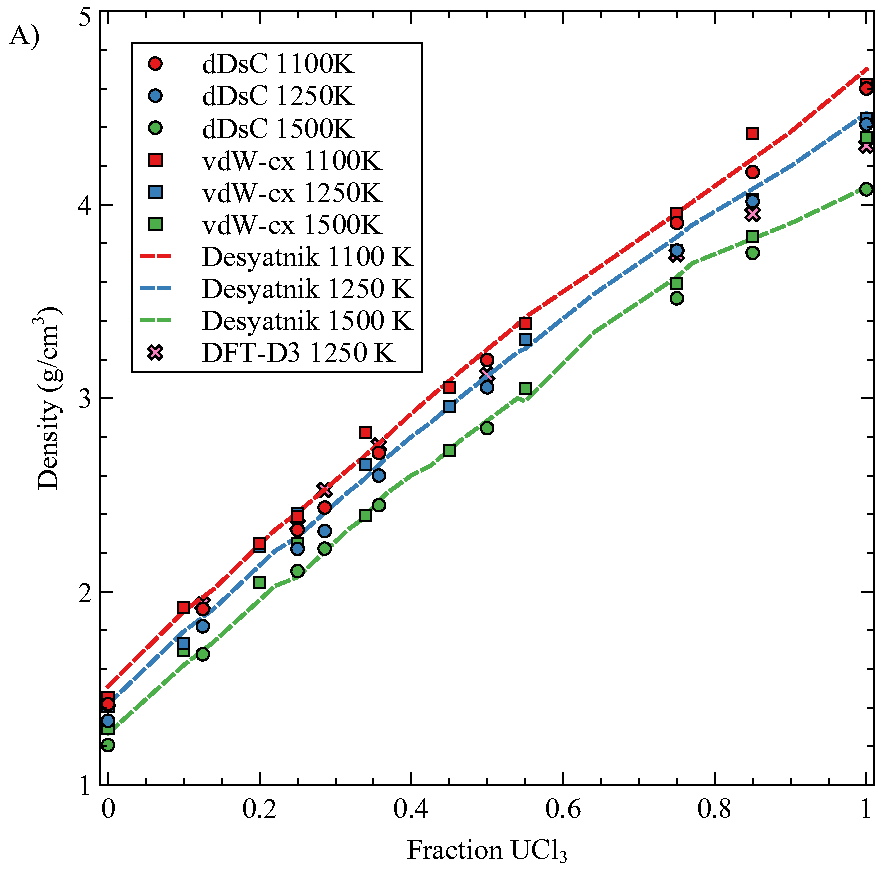
\includegraphics[width=0.45\textwidth]{ben_fig4a.pdf} 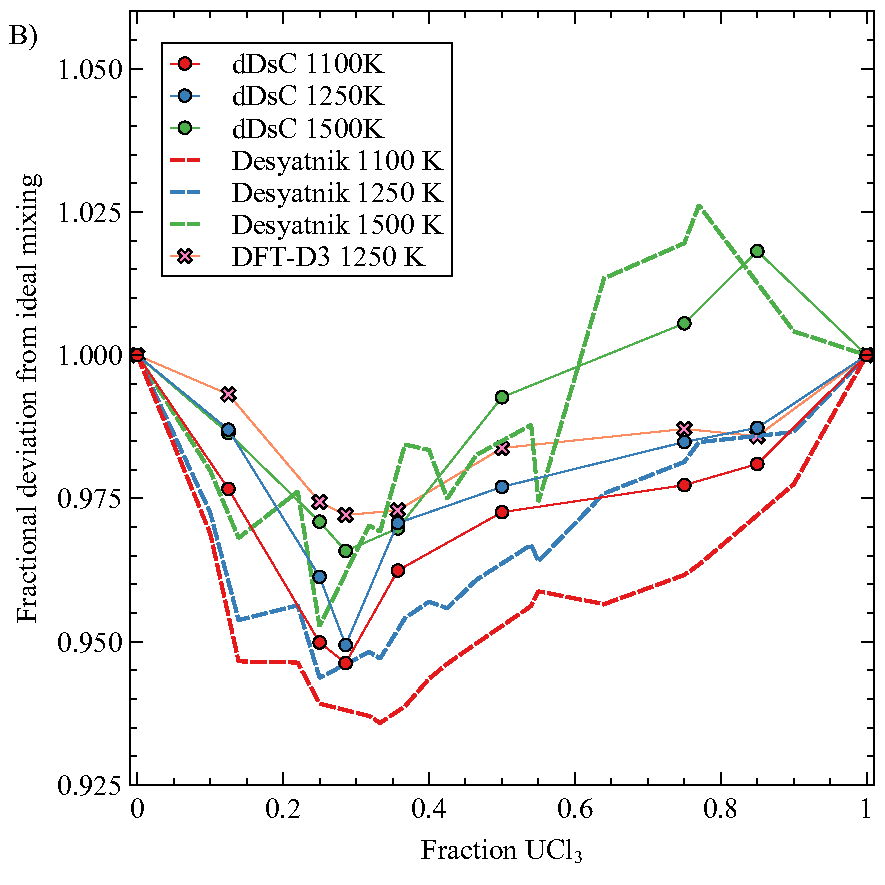
\includegraphics[width=0.45\textwidth]{ben_fig4b.pdf}
\caption{a) Densities of KCl-UCl$_3$ calculated from simulations using the (a) DFT-dDsC, vdW-cx, and DFT-D3 dispersion formulations. (b) The deviation from ideal solution behavior derived from the data in a). The correlations developed by Desyatnik \textit{et al.}~\cite{DesyatnikKCl} are represented by dashed lines in both figures.}
\label{fig:density}
\end{figure*}

Moon \textit{et al.}~\cite{Moon} performed neutron radiography measurements of the density of KCl-UCl$_3$ at two compositions, 22 and 57\% UCl$_3$. The results are shown in Figure \ref{fig:neutron}, which also contains estimates derived by interpolating the AIMD results for the compositions nearest to 22 and 57 \% UCl$_3$, respectively, from Desyatnik \textit{et al.}~\cite{DesyatnikKCl} using the same approach, and from the correlations derived by Can \textit{et al.}~\cite{agca2022}. The latter is primarily based on the data from Desyatnik \textit{et al.}~\cite{DesyatnikKCl}. Although the absolute density values in the temperature range investigated by experiments are close to the DFT-dDsC simulation results, while the vdW-cx results more closely match the data from Desyatnik. The slopes of both sets of AIMD data are closer to those reported by Desyatnik \textit{et al.}~\cite{DesyatnikKCl}, than the slope measured by Moon~\cite{Moon}. 
{\color{red} I commented out your last statement, as I think it changes now based upon my data. i think we can still have a sentence here, but I leave it to you to write, as my brain is getting fried.}
%In the temperature range of primary interest, the deviation between modeling and the radiography experiments~\cite{Moon} is less than the deviation between the data due to Desyatnik \textit{et al.}~\cite{DesyatnikKCl}.
In Figure \ref{fig:neutron}b, similar trends are shown with respect to the AIMD data sets, but the Moon measurements now show a non-linear thermal expansion, while still producing magnitudes similar to existing experimental data and the current computational data. 

\begin{figure*}[h!]
\centering
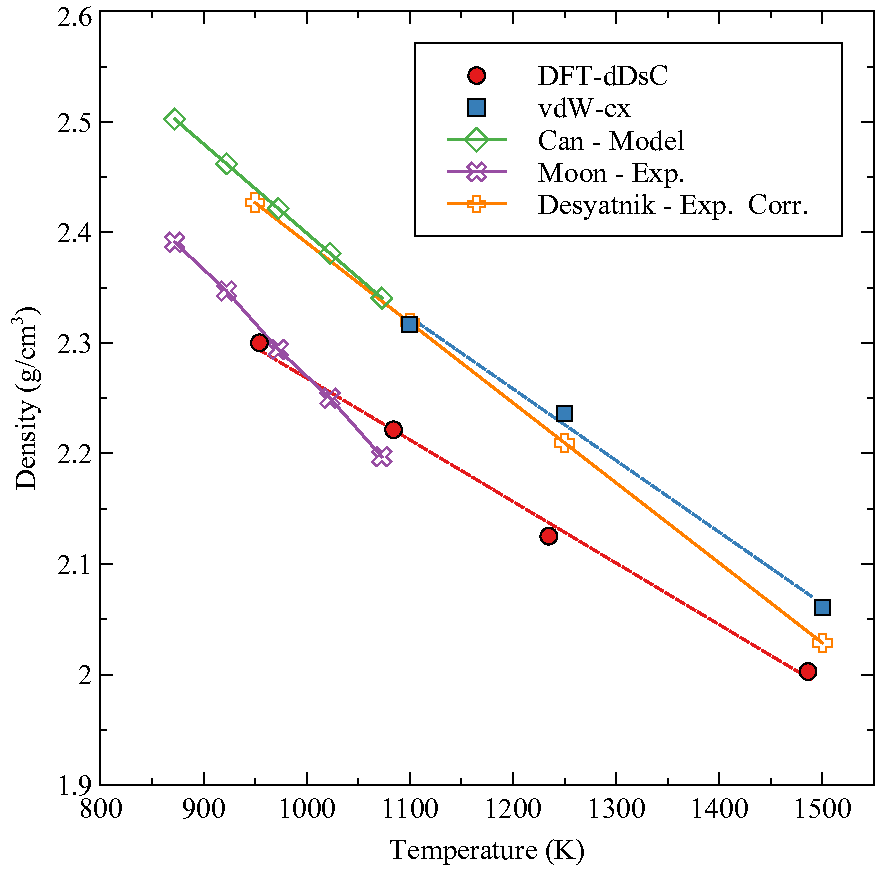
\includegraphics[width=0.45\textwidth]{ben_fig5a.pdf} 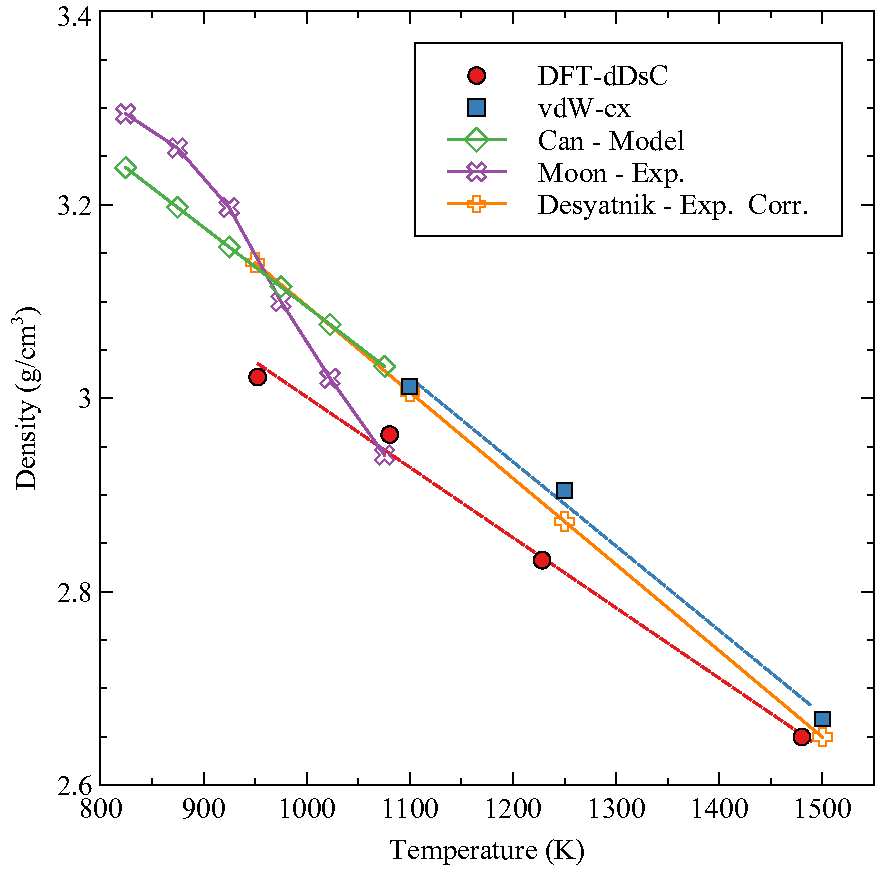
\includegraphics[width=0.45\textwidth]{ben_fig5b.pdf}
\caption{a) The density of 78\% KCl and 22\% UCl$_3$ as a function of temperature. Measurements were made by Moon et al.~\cite{Moon} and Desytanik et al.~\cite{DesyatnikKCl} (represented by the correlations derived from their measurements). The DFT-dDsC and vdW-cx data were obtained via interpolation of the studied compositions. b) The same information is in a) but for 57\% KCl and 43\% UCl$_3$. The dashed lines represent fits to the AIMD data points.}
\label{fig:neutron}
\end{figure*}

%\FloatBarrier

\subsection{Local structure-property correlations}
The AIMD simulations predict a minimum mixing energy close to 36 \% UCl$_3$, which is near, and likely corresponds to, the expected eutectic composition if the K$_2$UCl$_5$ phase could be suspended, thus confirming the observations for the NaCl-UCl$_3$ system. The density exhibits a maximum deviation from ideal solution behavior at approximately the same composition, though the maximum may be shifted to a slightly lower composition. Further, the mixing energy follows a linear trend between 0\% UCl$_3$ up to the eutectic composition of 36\%, after which it exhibits curvature up to pure UCl$_3$. This behavior is governed by the coordination chemistry of the solution phase. Studies by Li \textit{et al.}~\cite{Li} on NaCl-UCl$_3$ concluded that UCl$_3$ units form connected networks in the mixed salts above a concentration of 30\% UCl$_3$, and the UCl$_3$ units are more isolated below this concentration. These conclusions were later confirmed by Andersson \textit{et al.}~\cite{Andersson} by investigating the radial pair distribution function (RDF) as a function of composition. Between 36\% and about 100\% UCl$_3$, the U-U peak in NaCl-UCl$_3$ stays remarkably constant, while below the 36\% value, it starts to change significantly, which is an indication of the network structure breaking up. Initial signs of the break up occur between 36 and 50\% UCl$_3$. Related changes may be observed in other distribution functions. In addition, it was proposed that between 0 and 36\% UCl$_3$, the mixture attempts to partially phase separate into NaCl and the eutectic mixture, which was supported by analysis of the pair distribution function (mimicking the UCl$_3$ case) and the mixing energy (almost a linear relations in-between these compositions). This is an intriguing observation, however, it should be noted that the supercells are too small to draw strong conclusions, and the sampling in the time domain could also impact the results. 

The corresponding radial pair distribution functions for KCl-UCl$_3$ at 1250 K are shown in Figure \ref{fig:fig_pair}. The RDFs and the composition dependence confirm that the analysis for NaCl-UCl$_3$ also applies to KCl-UCl$_3$, which is consistent with the two systems exhibiting similar trends for density and mixing energies. To reiterate the observation for NaCl-UCl$_3$~\cite{Andersson}, starting from the UCl$_3$ end-member, the negative mixing energy is a consequence of incorporating the KCl units within the UCl$_3$ network, however, once the UCl$_3$ concentration is below $\approx36\%$, lowering of the mixing energy by incorporating additional KCl units is countered by not maintaining the favorable U-U coordination seen in UCl$_3$, as evidenced by the U-U radial distribution function starting to significantly deviate from the UCl$_3$ reference case. This is equivalent to the break-up of the UCl$_3$ network structure. Figure \ref{fig:fig_pair}e) indicates that break-up occurs between 36\% and 50\% UCl$_3$. Similar to NaCl-UCl$_3$, it is believed that the linear trend for the mixing energy between 0\% and 36\% UCl$_3$ is indicative of a partial phase separation to take advantage of the favorable interactions close to the 36\% UCl$_3$ composition. However, it must be acknowledged that the small size of the current simulation cells limits the ability to draw strong conclusions. 

\begin{figure*}[h!]
\centering
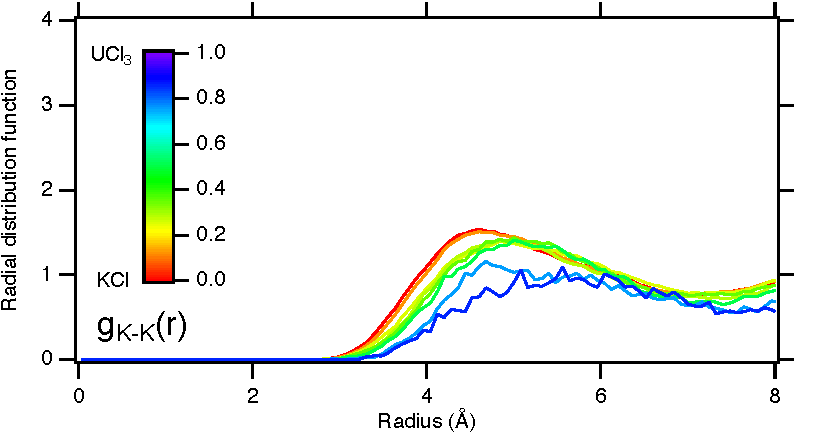
\includegraphics[width=0.33\textwidth]{rdf1.pdf}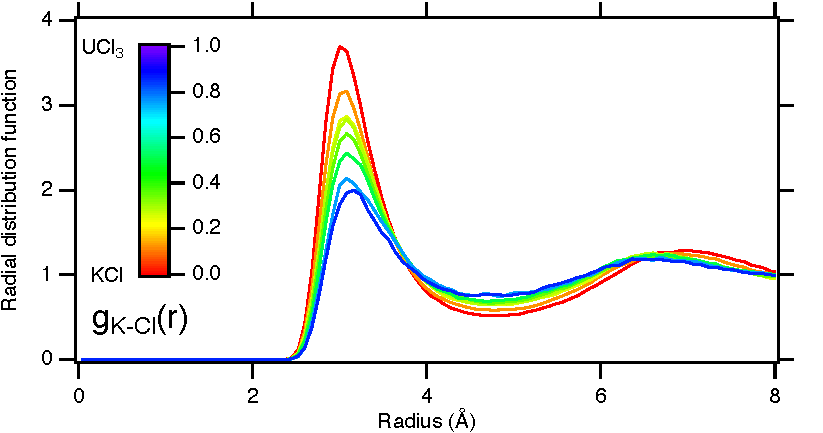
\includegraphics[width=0.33\textwidth]{rdf2.pdf}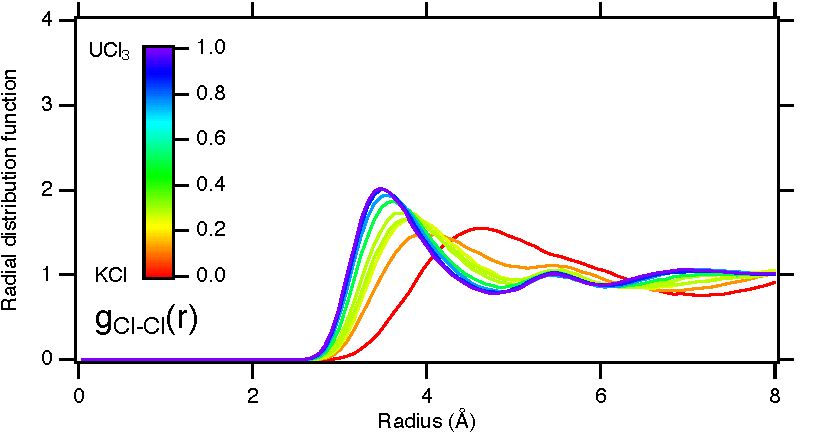
\includegraphics[width=0.33\textwidth]{rdf3.pdf}
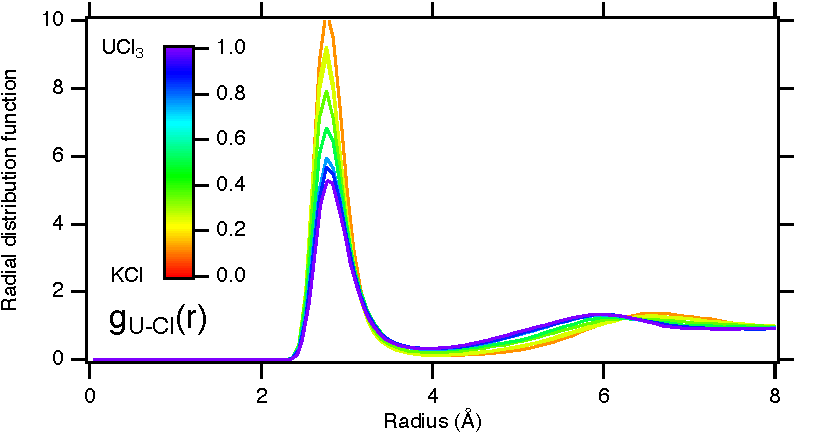
\includegraphics[width=0.33\textwidth]{rdf4.pdf}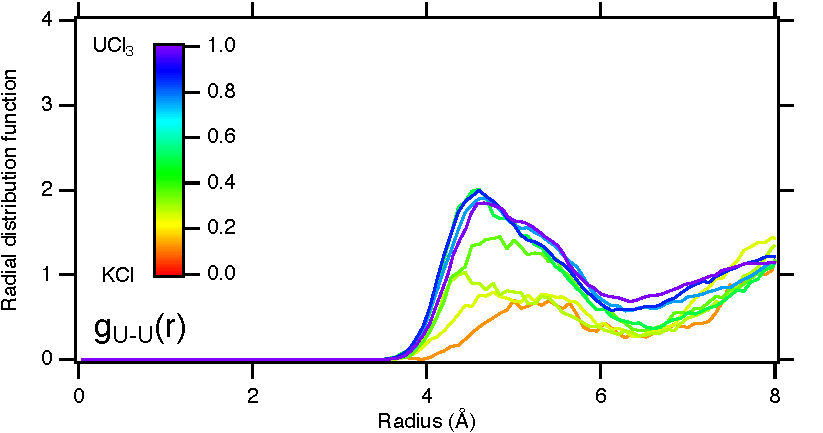
\includegraphics[width=0.33\textwidth]{rdf5.pdf}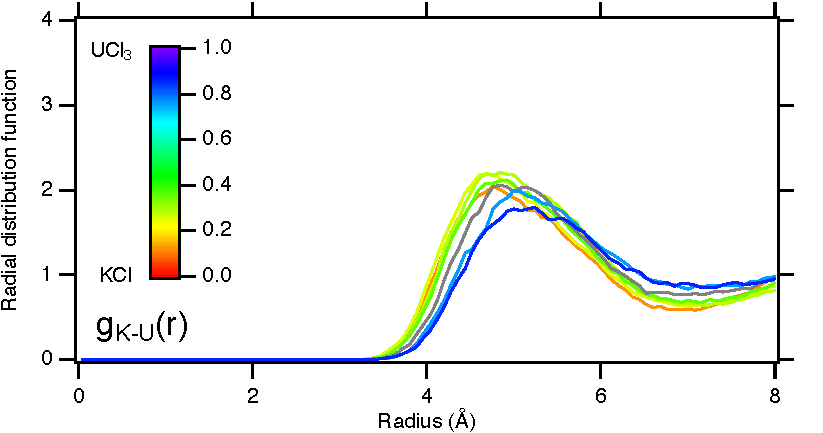
\includegraphics[width=0.33\textwidth]{rdf6.pdf}
\caption{Partial radial pair distribution functions for KCl-UCl$_3$ mixtures. a) K-K, b) K-Cl, c) Cl-Cl, d) U-Cl, e) U-U and f) K-U.} 
\label{fig:fig_pair}
\end{figure*}

\section{Conclusions}
\label{sec:conclusions}
AIMD simulations were performed on the KCl-UCl$_3$ molten salt system to predict temperature-dependent thermodynamic (mixing energy and heat capacity) and thermophysical (density and thermal expansion) properties. Several different models for dispersion force interactions were investigated. The results show heat capacities and mixing energies in qualitative agreement with experimental data. The mixing energies are negative with a minimum close to 36 \% UCl$_3$. This composition coincides with the breakup of UCl$_3$ network structures in the liquid solution phase, which is consistent with existing observations for related systems (NaCl-UCl$_3$). The simulations did not reveal a clear temperature dependence for the mixing energy. Density is predicted to have a negative deviation from ideal solution behavior with a weak temperature dependence, though close to the UCl$_3$ end-member composition the deviation turns positive at high temperatures. The largest deviation from ideal solution occurs near the composition of the maximum mixing energy, however, it is slightly shifted towards the KCl end-member. The magnitude of the mixing densities and the trends are in qualitative agreement with available experiments, though some disagreement exists at the quantitative level. Compared to the previously studied NaCl-UCl$_3$ system, mixing energies and densities are about twice as large, which is consistent with empirical correlations based on ionic sizes. 


\section*{Acknowledgements}
This work was funded by the U.S. Department of Energy (DOE), Office of Nuclear Energy, Nuclear Energy Advanced Modeling and Simulation (NEAMS) program, and the INL Laboratory Directed Research and Development (LDRD) Program. Los Alamos National Laboratory, an affirmative action/equal opportunity employer, is operated by Triad National Security LLC, for the National Nuclear Security Administration of the U.S.\ Department of Energy under Contract No. 89233218CNA000001. Idaho National Laboratory is operated by Battelle Energy Alliance, LLC with the U.S. Department of Energy under Contract No. DE-AC07-05ID14517. This research made use of the resources of the High-Performance Computing Center at Idaho National Laboratory, which is supported by the Office of Nuclear Energy of the U.S. Department of Energy and the Nuclear Science User Facilities.       


\bibliographystyle{elsarticle-num} 
\bibliography{Yellowjacket.bib}

\end{document}

